\chapter{Implementation}\label{ch:implementation}
%The purpose of this chapter is, on the one hand, to make it credible that you are not dealing with a "paper tiger" but with a real existing system. It is certainly also a very important text for someone who will continue the work later. The third aspect is to give the reader a deeper impression of the technology that is being dealt with here. Nice examples are "War Stories", i.e. things you had to struggle with in particular. (5-20 pages)

In the following sections, I will demonstrate the implementation of the described design on the Versal platform. The use of the Xilinx toolchain and the general workflow will be outlined. Additionally, the development and implementation of test cases will be discussed, including the generation of test data for these cases.

\section{Implementation on the Versal}\label{sec:imp}
Before delving into the specifics of the implementation, an overview of the Xilinx toolchain is necessary to understand how certain implementation decisions are shaped by the build process. The toolchain primarily consists of the Xilinx v++ compiler and linker \cite{churiwala_designing_2017}. The compiler is used to compile code for the AI engines and to generate the hardware description for the \ac{pl} via high-level synthesis. This process is completed in two steps: first, generating a VHDL file from a C++ design description, and second, compiling this VHDL representation into a .xo hardware file. This approach enables potential VHDL-level optimizations without requiring the design to be rewritten entirely from scratch. The v++ linker then connects and links the AI engine binary with the \ac{pl} description into a single .xsa container file, which can be loaded onto the Versal platform to configure both the \ac{pl} and AI engines. Command-line tools are used to interact with these processes, which can be integrated into a makefile to manage the build sequence. This setup allows for a modularized build process and provides the ability to examine the effects of specific compile flags at each stage.\par
In addition to creating the hardware description container, an application is required to invoke the configured hardware. This application can either be implemented as a bare-metal application or a Linux user-space application. For the latter, a Linux installation on the ARM host system and a compatible compiler are necessary. Implementing the application on Linux is advantageous because it enables the use of existing infrastructure, such as drivers, for interaction with the hardware container. The Linux build system, YOCTO, is employed to acquire the Linux image and set up the configured compiler. YOCTO facilitates the creation of an image and a cross-compiler toolchain with all essential packages and headers \cite{streif_embedded_2016}. In this project, a Linux image and a compiler with the Asio C++ library for networking, generated by YOCTO, are utilized.\par
Once all components are created, they are combined into a single image that can be deployed to the Versal platform. This package is generated by the v++ linker and can include additional files, which will be transferred to the board's memory. This feature is particularly useful for transferring data files to the test environment.

\subsection{Integration of the AI Engine kernel} \label{sec:aie_im}
As previously mentioned, the kernel is implemented in C++ using the Xilinx-specific compiler. Before detailing the complete kernel implementation, I will first describe the implementation of the 256-point \ac{fft}, as it serves as the core functionality of the kernel. The 256-point \ac{fft} is structured as a simple, non-inlined function. This decision stems from the limited program memory available on a single AI Engine tile. However, to reduce function call overhead, all functions within the \ac{fft} are inlined. This approach results in a single code block containing the complete \ac{fft}, which can be entered and exited with one \texttt{jmp} instruction. Consequently, the \ac{fft} function is named \texttt{not\char`_inline\char`_256\char`_FFT}.\par
Within this function, there are multiple calls to different implementations of a function called \texttt{radix\char`_4\char`_stage}. They range from zero to three, representing the four \ac{fft} stages described in section \ref{sec:design_ai}. These stages are abstracted into separate functions, enabling flexibility for future modifications, such as adding or removing stages. Each function is similar in structure, with slight variations tailored to each stage. I will first outline the general structure, as it is consistent across each function. Generally, the functions accept four cfloat pointers as input: two pointing to the input and output buffers, and the other two pointing to lookup tables—one for twiddle factors within the \ac{fft} stage and the other for phase rotation. All functions utilize the radix-4 \ac{fft}, so the first lookup table consistently uses the same pointer to the radix-4 lookup table. The general structure of the algorithm is depicted as pseudo-code in \ref{alg:FFT}.\par
The radix-4 \ac{fft} is implemented using the \texttt{fpmac} intrinsic provided by the AI Engine \cite{AMD_aie_intrinsics}. This intrinsic performs a multiply-and-add operation on two input vectors of four elements each within two clock cycles. To implement the four-point \ac{fft}, the \texttt{fpmac} operation is invoked four times, acting on four elements of the input vector and the twiddle factor lookup table. During these calls, the element order for multiplication and addition is adjusted to model the entire \ac{fft}. This approach reduces the \ac{fft} cycle count from 32 cycles (16 for multiplication and 16 for addition) to 8 cycles for the four \texttt{fpmac} calls. Following this, a vector multiplication (\texttt{fpmul}) with the second lookup table is applied to the result vector to complete the phase rotation.\par
For these vector operations, the relevant sections of the buffer and lookup tables must be loaded into the vector registers, as described in section \ref{sec:versal}. Consequently, two load operations are executed before each \texttt{fpmac} and \texttt{fpmul} operation. To minimize loading overhead, the input buffer is divided into four segments, which are loaded into the vector register simultaneously. This creates a loop where four four-element vectors are loaded into the vector register. The \texttt{fpmac} operations for the \ac{fft} are then executed on these preloaded vectors, and phase rotation is subsequently applied to the results. This loop continues until every element of the output buffer has been calculated. For each of the aforementioned \ac{fft} stages, the size of the segmented input buffer and, therefore, the loop iterations vary, which necessitates distinct functions for each stage. The general structure is shown in the following pseudo-code while figure \ref{fig:vector_load} shows the utilization of the vector unit.\par

\begin{algorithm}
\caption{FFT Implementation} \label{alg:FFT}
\begin{footnotesize} % Reduzierte Schriftgröße
\begin{algorithmic}
\STATE \textbf{Function} \textit{not\_inline\_256\_FFT}(input\_buffer, output\_buffer, tw\_lut, ph\_lut)
    \STATE \hspace{0.3cm} \textbf{for each} stage in \{0, 1, 2, 3\} \textbf{do}
    \STATE \hspace{0.6cm} \textit{radix\_4\_stage}(input\_buffer, output\_buffer, tw\_lut, ph\_lut, stage)
    \STATE \hspace{0.3cm} \textbf{end for}
    \STATE \hspace{0.3cm} \textit{reorder\_output}(output\_buffer)
\STATE \textbf{End Function}

\STATE \textbf{Function} \textit{radix\_4\_stage}(input\_buffer, output\_buffer, tw\_lut, ph\_lut, stage)
    \STATE \hspace{0.3cm} \textbf{for each} seg in in\_buf \textbf{do}
    \STATE \hspace{0.6cm} Load seg into vector register
    \STATE \hspace{0.6cm} \textbf{for} i = 1 to 4 \textbf{do}
    \STATE \hspace{0.9cm} Perform \textit{fpmac} with tw\_lut and input vec
    \STATE \hspace{0.6cm} \textbf{end for}
    \STATE \hspace{0.6cm} Perform \textit{fpmul} with ph\_lut for phase rotation
    \STATE \hspace{0.3cm} \textbf{end for}
\STATE \textbf{End Function}

\STATE \textbf{Function} \textit{reorder\_output}(output\_buffer)
    \STATE \hspace{0.3cm} Reorder elements in out\_buf for sequential loading
\STATE \textbf{End Function}
\end{algorithmic}
\end{footnotesize}
\end{algorithm}


\begin{figure}[h]
    \centering
    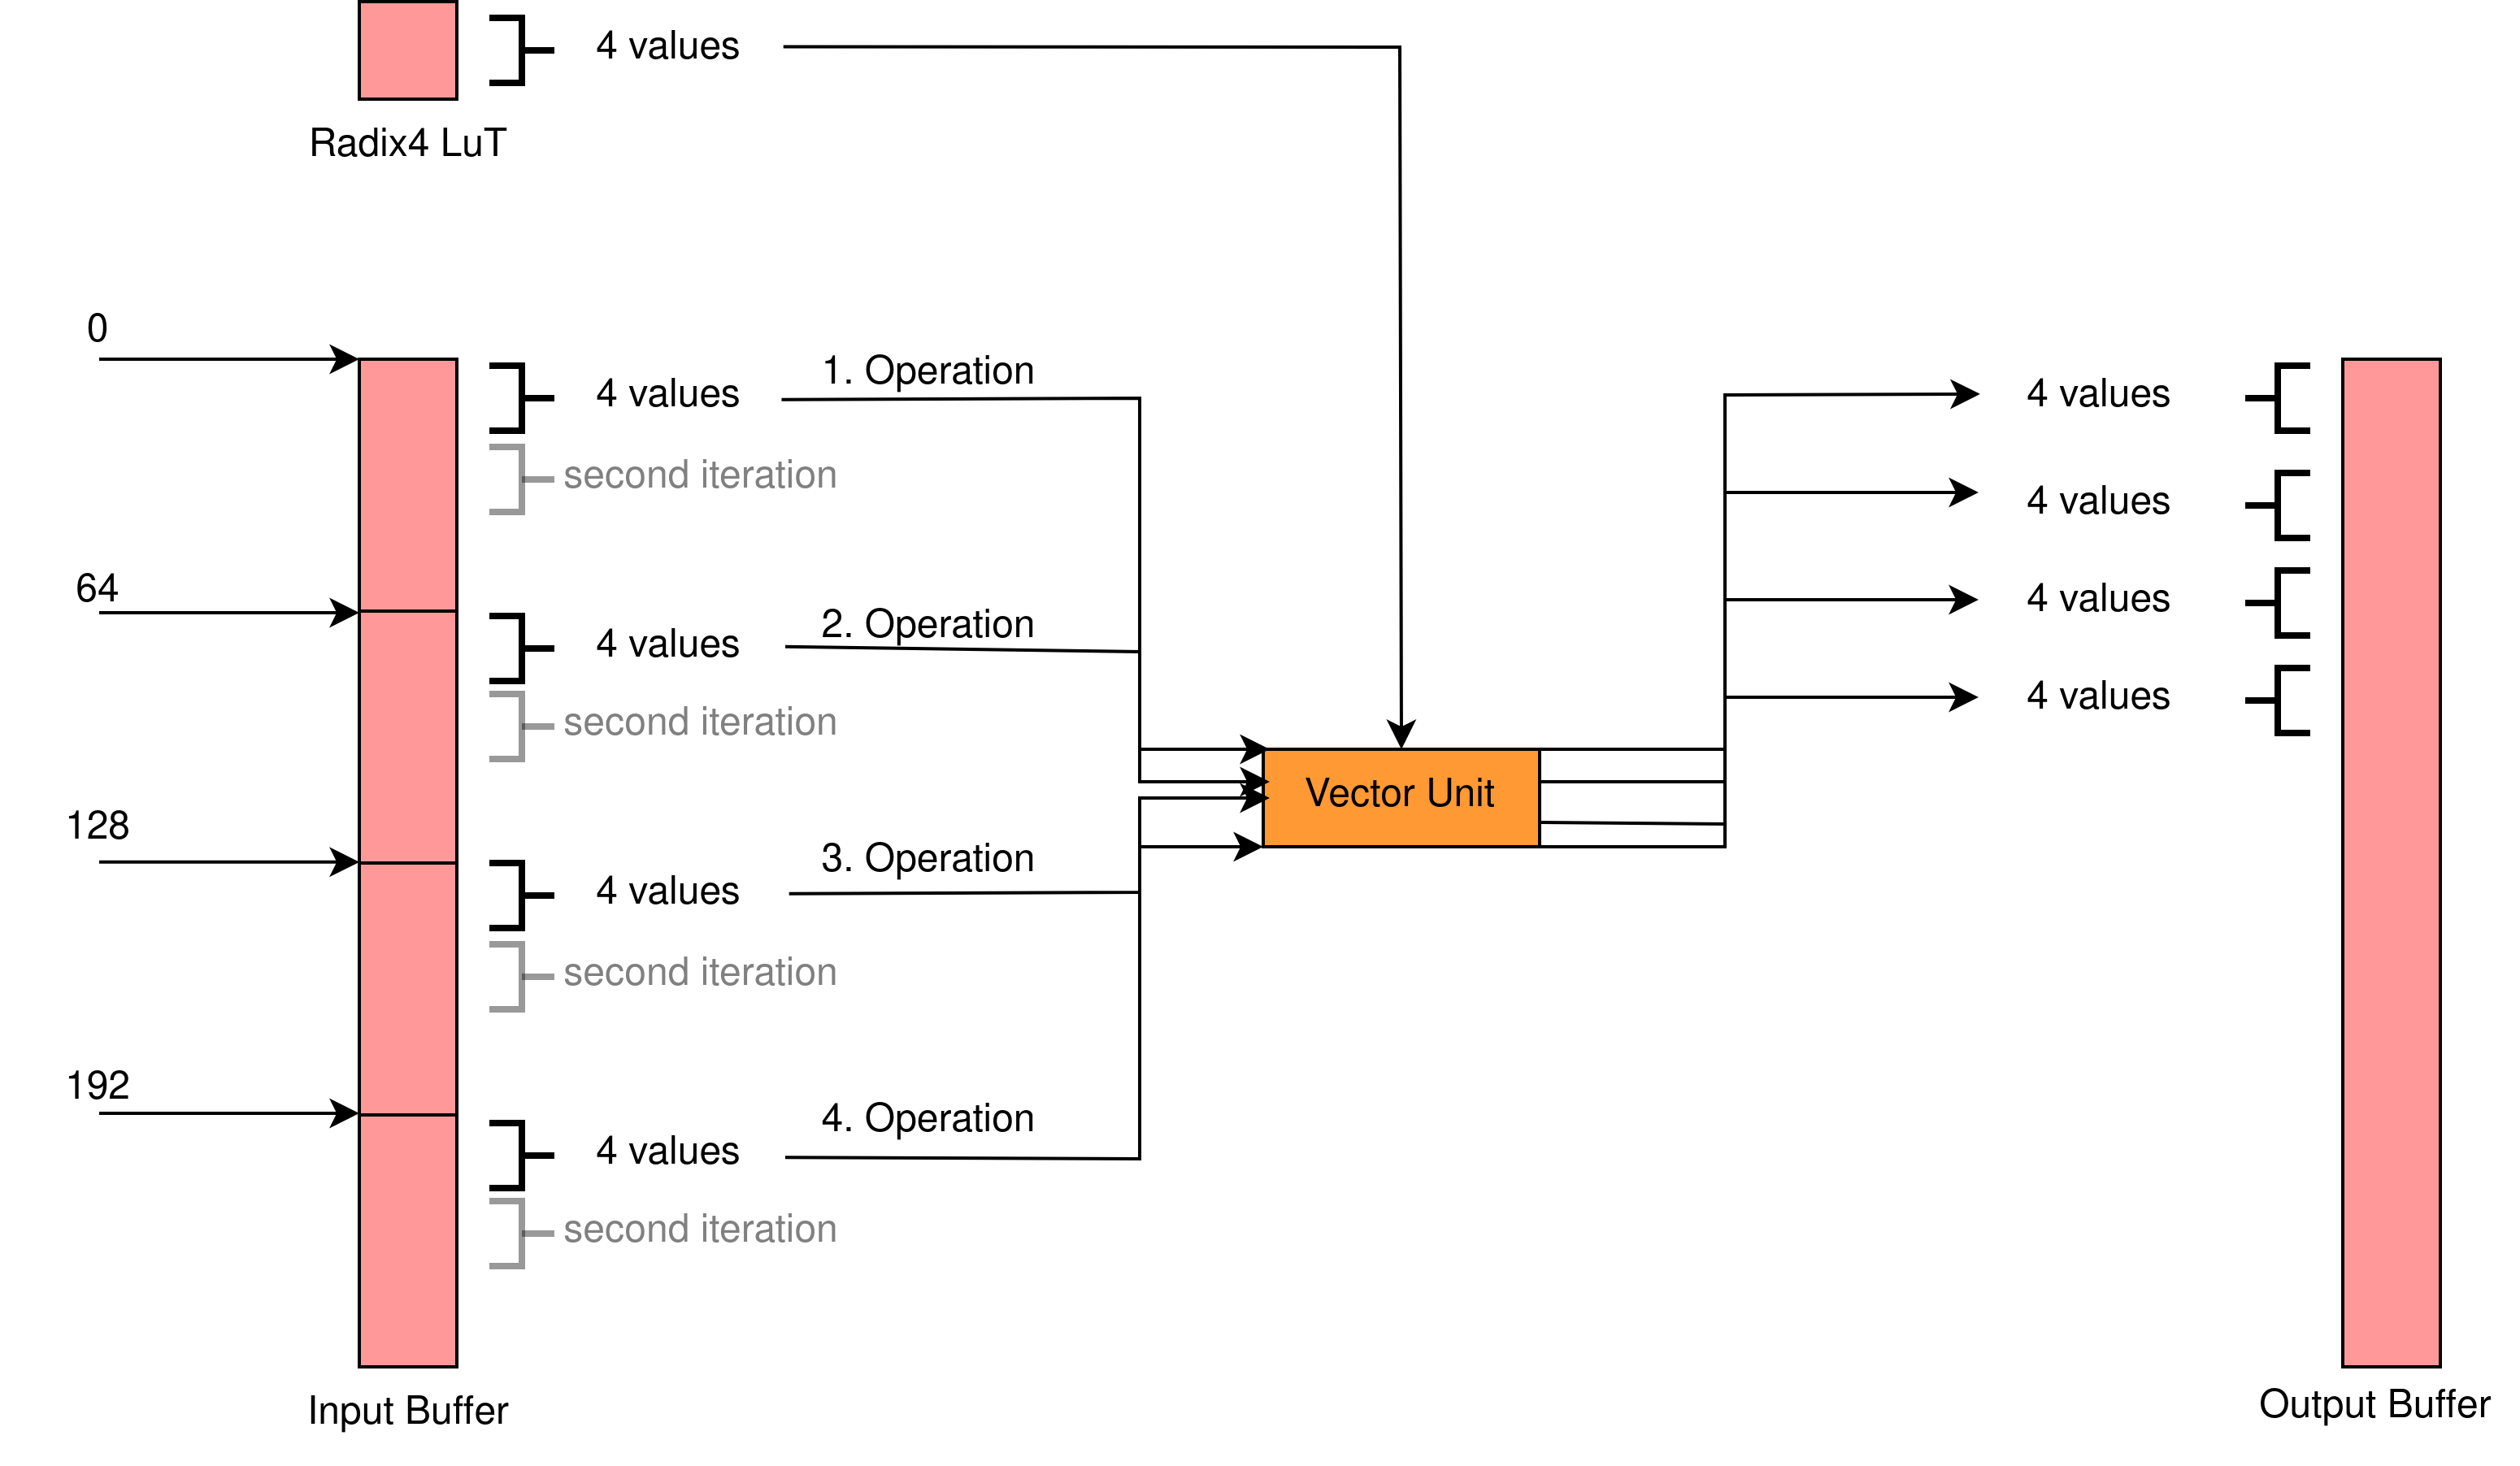
\includegraphics[width=1.0\textwidth]{images/vector_load.png}
    \captionsetup{justification=centering}
    \caption{Load order for the vector unit}
        Memory loads from the memory banks in red to the vector registers in orange during multiple iterations of the radix-4 functions. One load to each 64 value block of the input buffer is done during every iteration. 
    \label{fig:vector_load}
\end{figure}

Between the different \ac{fft} stages, a reorder function is used to enable sequential element loading from the buffer into the vector unit, thereby minimizing and accelerating read and write operations. Like the other functions, these reorder functions are inlined to contribute to the monolithic \texttt{not\char`_inline\char`_256\char`_FFT} code block. \par
Having discussed the construction of the main \ac{fft} function, I will now describe the complete kernel. The kernel function operates on two cfloat buffers, each containing 1024 elements for input and output. Each buffer occupies one memory rank of the AI Engine tile’s buffer. To ensure memory alignment, the control word, which configures the kernel, must also fit within this buffer. A simple yet effective solution is to place this control word within the data frame, as the initial input for the first stage of the $2^{18}$-point \ac{fft} is real-valued, requiring the same buffer as the complex-valued input of the second stage. Therefore, the complex components of the input buffer remain unused. The control word is intentionally designed to be an invalid floating-point value, which the kernel can identify. The kernel operation checks whether the first complex value in the input buffer is NaN. If so, the kernel is set up for the first stage, and the first complex value is reset to zero. If the value is valid, the kernel is set up for the second stage, and no changes are made to the data frame. In both configurations, the \texttt{not\char`_inline\char`_256\char`_FFT}function is called four times on different segments of the data frame. Data frame access is managed through four pointers, each pointing to a different 256-point segment. Intermediate results between \ac{fft} stages are stored in the output buffer, which is only streamed when its final element is written. To avoid filling the output buffer, an additional 256-element buffer is used. If the kernel is configured for the first stage, a phase rotation is applied afterward using the \texttt{fpmul} operation described earlier. Each kernel instance has a unique phase rotation lookup table, assigned through preprocessor directives. The complete kernel is generated as a macro, invoked before compilation to create kernel functions with distinct lookup tables.\par
To define the data paths between kernels, a directed graph is used, as outlined in section \ref{sec:versal}. Each class capable of sending or receiving data includes input, output, or both types of ports, which can be connected to represent directed data streams. Thus, only output-to-input connections are valid. The kernel function described above is instantiated within a kernel class, which calls this function internally. The size of the input buffer dictates the number of elements that must be streamed to the input port before invoking this function, which, in this case, requires exactly 1024 elements. Failure to stream this quantity will result in a system crash. The general memory utilization is shown in figure \ref{fig:memory_structure}. \par
For this design, multiple input streams are defined and exposed to the \ac{pl}. This is achieved using the \texttt{input\char`_plio} and \texttt{output\char`_plio} classes, which serve as abstractions for connection tiles. The \texttt{pktsplit} class is used to divide the eight input streams into 32 data packets, mimicking the routing hardware's split mechanism. This class has one input port and a maximum of 32 output ports. Each \texttt{input\char`_plio} output port connects to a \texttt{pktsplit} input port, and each \texttt{pktsplit} output port connects to an individual kernel instance input port. This design employs 256 kernel instances. For the reverse flow, to merge data back into the \ac{pl}, the \texttt{pktmerge} class is used. Acting as the \texttt{pktsplit} counterpart, it accepts 32 inputs and merges them into a single output stream, meaning that 32 kernel instances connect to one \texttt{pktmerge}, which in turn connects to an \texttt{output\char`_plio}. This allows to only use eight of the connection tiles of the AI Engine array. In consequence the \ac{pl} kernel only need to deal with eight streams which reduces the overhead.\par
In addition to the input and output ports, each kernel can also have multiple parameter ports, which can connect to lookup tables. For this design, each kernel includes six parameter ports connected to lookup tables for the different \ac{fft} stages. These lookup tables are defined as arrays and are automatically generated by a Python script. During compile time they are assigned to a memory location within the AI Engine memory block.

\begin{figure}[h]
    \centering
    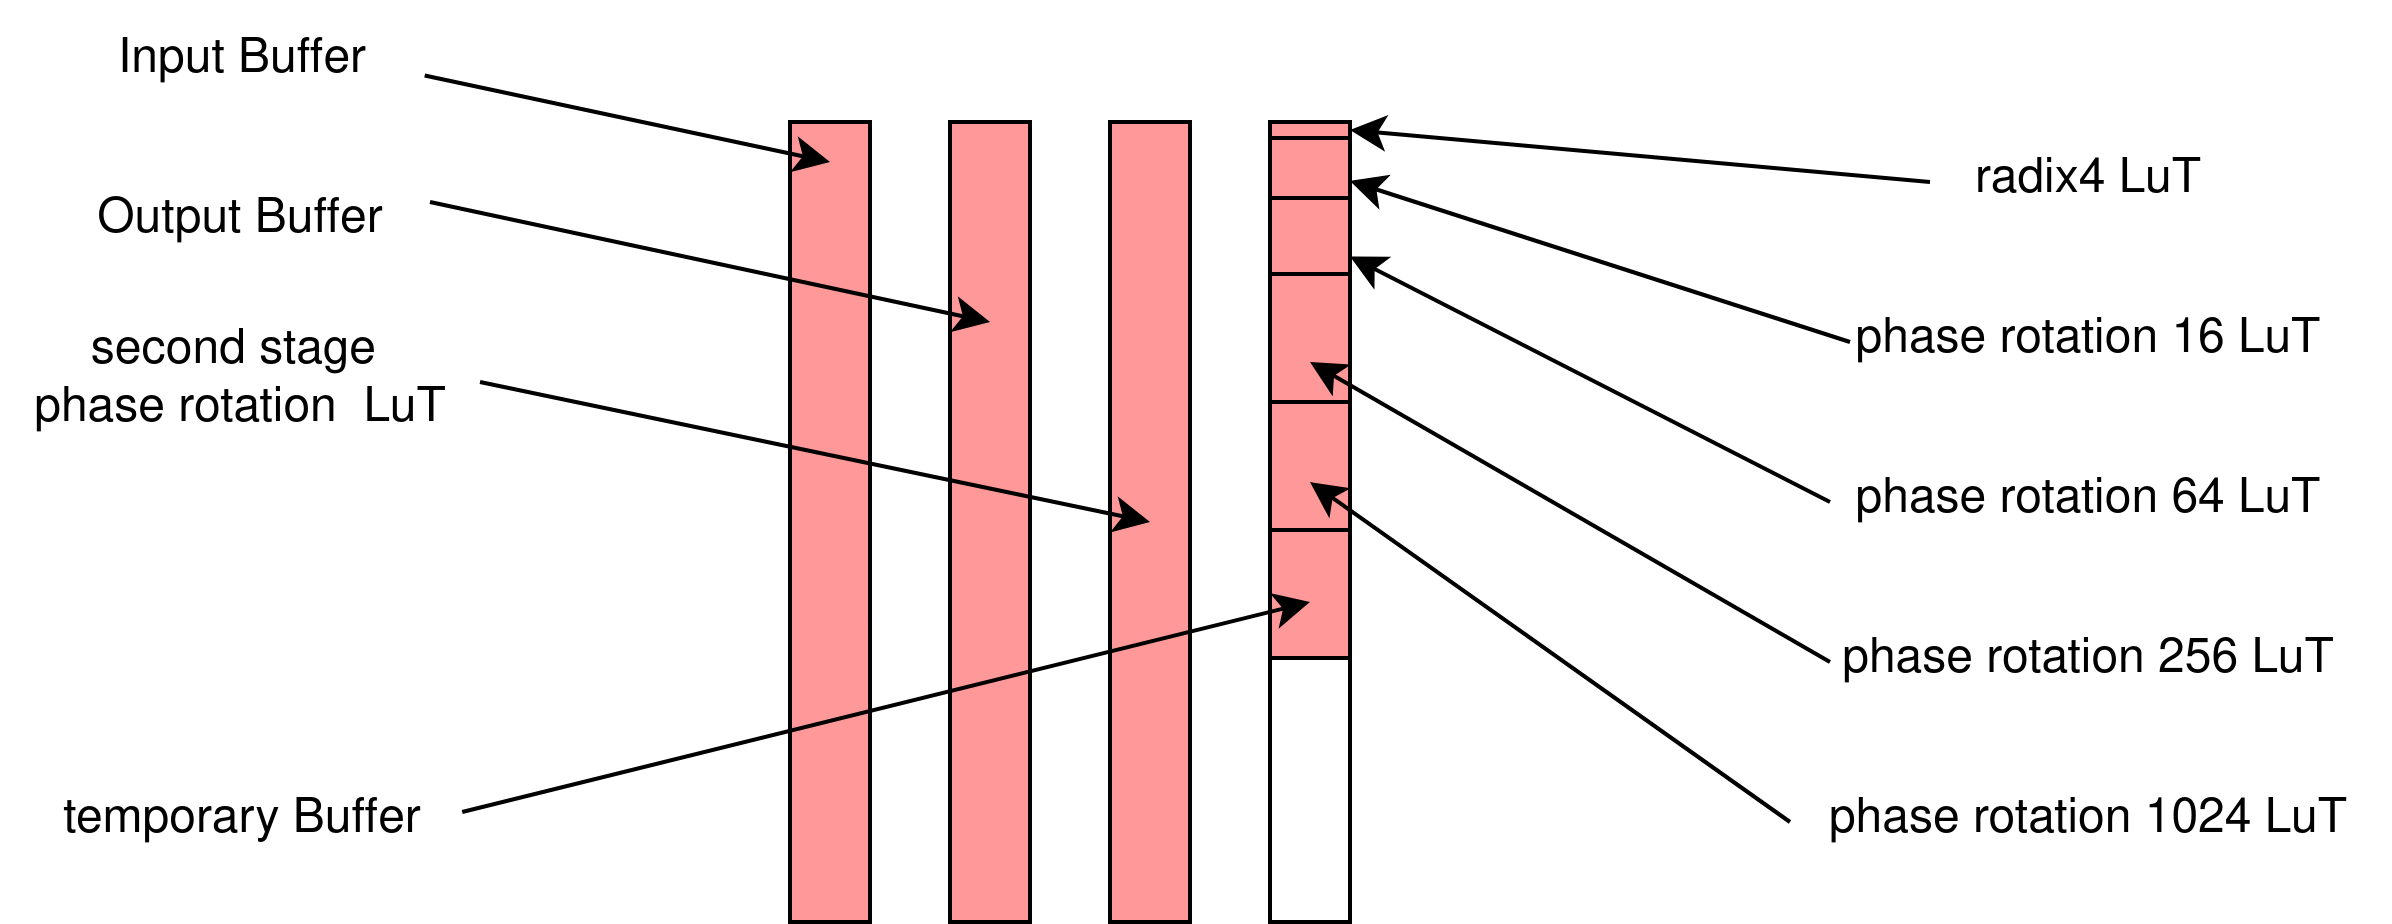
\includegraphics[width=1.0\textwidth]{images/memory_structure.png}
    \captionsetup{justification=centering}
    \caption{Occupied memory banks of the 32 kb AI Engine memory}
        The memory utilization of every single memory bank. Red shows the alocated memory split into its use cases.
    \label{fig:memory_structure}
\end{figure}

\subsection{Construction of the programmable logic}
As previously described, the \ac{pl} is defined using high-level synthesis \cite{coussy_introduction_2009} in C++. Kernels within the \ac{pl} are defined as functions specifying the kernel’s functionality. Consequently, the reorder mechanisms across kernels are implemented as simple loops that write values into an array in the correct order. These values are then read from the array and sequentially streamed between kernels.\par
Several points require special consideration in this setup. First, the use of arrays: unlike in a conventional program, arrays in this context do not lead to RAM memory allocation, as the \ac{pl} lacks such memory. Instead, the array is implemented in \ac{pl} using available block RAM. This allows faster access as the memory is directly connected to the streams and does not have an virtualisation layer between these two components. On the other hand it necessitates careful considerations regarding the size of certain buffers as memory can not be allocated or swapped out easily. The current design lead to an allocation of 63 percent of the available block RAM resources and 27 percent allocation of the available LuT resources.  Another essential point is the handling of streams between \ac{pl} kernels and between these kernels and the AI Engines. Streams between kernels are initiated as arguments in the function defining a kernel. For this implementation, AXI streams are used, as they also provide compatibility with the AI Engines without requiring protocol modifications. Xilinx's AXI implementation offers both blocking and non-blocking read and write operations for streams. With blocking reads, writes are only executed once reads from all streams are completed. This could pose an issue for the design, specifically in a kernel with multiple input streams, where not all streams are active simultaneously. For example, the Packetsender kernel can receive streams from either the Partitioner or the Reorderer. To accommodate this, it includes eight streams connected to the Partitioner and eight connected to the Reorderer. A blocking read would delay all writes until data from all 16 streams is read. To avoid this, the non-blocking variant is used, allowing synchronization concerns to be managed by buffering data in an array beforehand.\par
The methods chosen to implement \ac{pl} kernels enable a straightforward and efficient design, allowing more focus on the overall structure and the AI Engines, which are the primary focus of this work.\par

\subsection{Host application}
The host application runs on the ARM processor and manages both the AI Engines and the \ac{pl}. From the host application’s perspective, the \ac{pl} and AI Engines act as accelerators to which tasks can be delegated, following a target-offloading approach. The application runs in userspace on a Linux operating system, enabling userspace drivers to interact with the hardware as shown in figure \ref{fig:host_interact}. Xilinx provides the Xilinx Runtime (XRT) \cite{xrt}, a user-kernel driver combination, to facilitate this interaction. One of XRT’s key functions is loading a hardware container, which is the linked result of the AI Engine and \ac{pl} kernels, and configures the hardware with the programmed functionality. The XRT’s load function flashes this container onto the hardware.\par
Once configured, the AI Engines and \ac{pl} functionalities are called using different methods. For \ac{pl} kernels that interact with DDR memory, memory must be allocated and passed to the kernel. The kernel can then be activated by calling it as a function, after which it starts running as soon as data is written to its memory location. Other \ac{pl} kernels operate similarly, starting execution upon receiving data from a stream. The AI Engine graph, however, is instantiated as a class with various callable functions. The graph is initialized with \texttt{graph.init()} and started with \texttt{graph.run()}. Like the \ac{pl} kernels, the AI Engines begin execution when data is streamed to the connection tiles. The \texttt{run()} function accepts an argument specifying the number of graph run repetitions. For example, passing \texttt{1} means the graph will execute once, and if data continues to stream afterward, the engines will stall. In this design, two calls to the AI Engines are made, one for the first \ac{fft} stage and one for the second, so \texttt{graph.run(2)} is used. Upon completing both runs, resources are released with \texttt{graph.end()}.\par
With the management of \ac{pl} and AI Engines from the host application described, an overview of data loading and result processing is provided here. The algorithm’s input data is initially read from a text file and copied to memory allocated for the Partitioner. After execution, results are retrieved from memory allocated for the Collector and saved to an output file. These results are used to calculate the root mean square error (RMSE) by comparing them to precomputed correct values from another file. All of these steps take place locally on the Versal platform. To transfer results to another system for further analysis, a network connection is established using the Asio C++ library. The following section will delve into the generation of test data and the computation of the correct results used as the ground truth.\par

\begin{figure}[h]
    \centering
    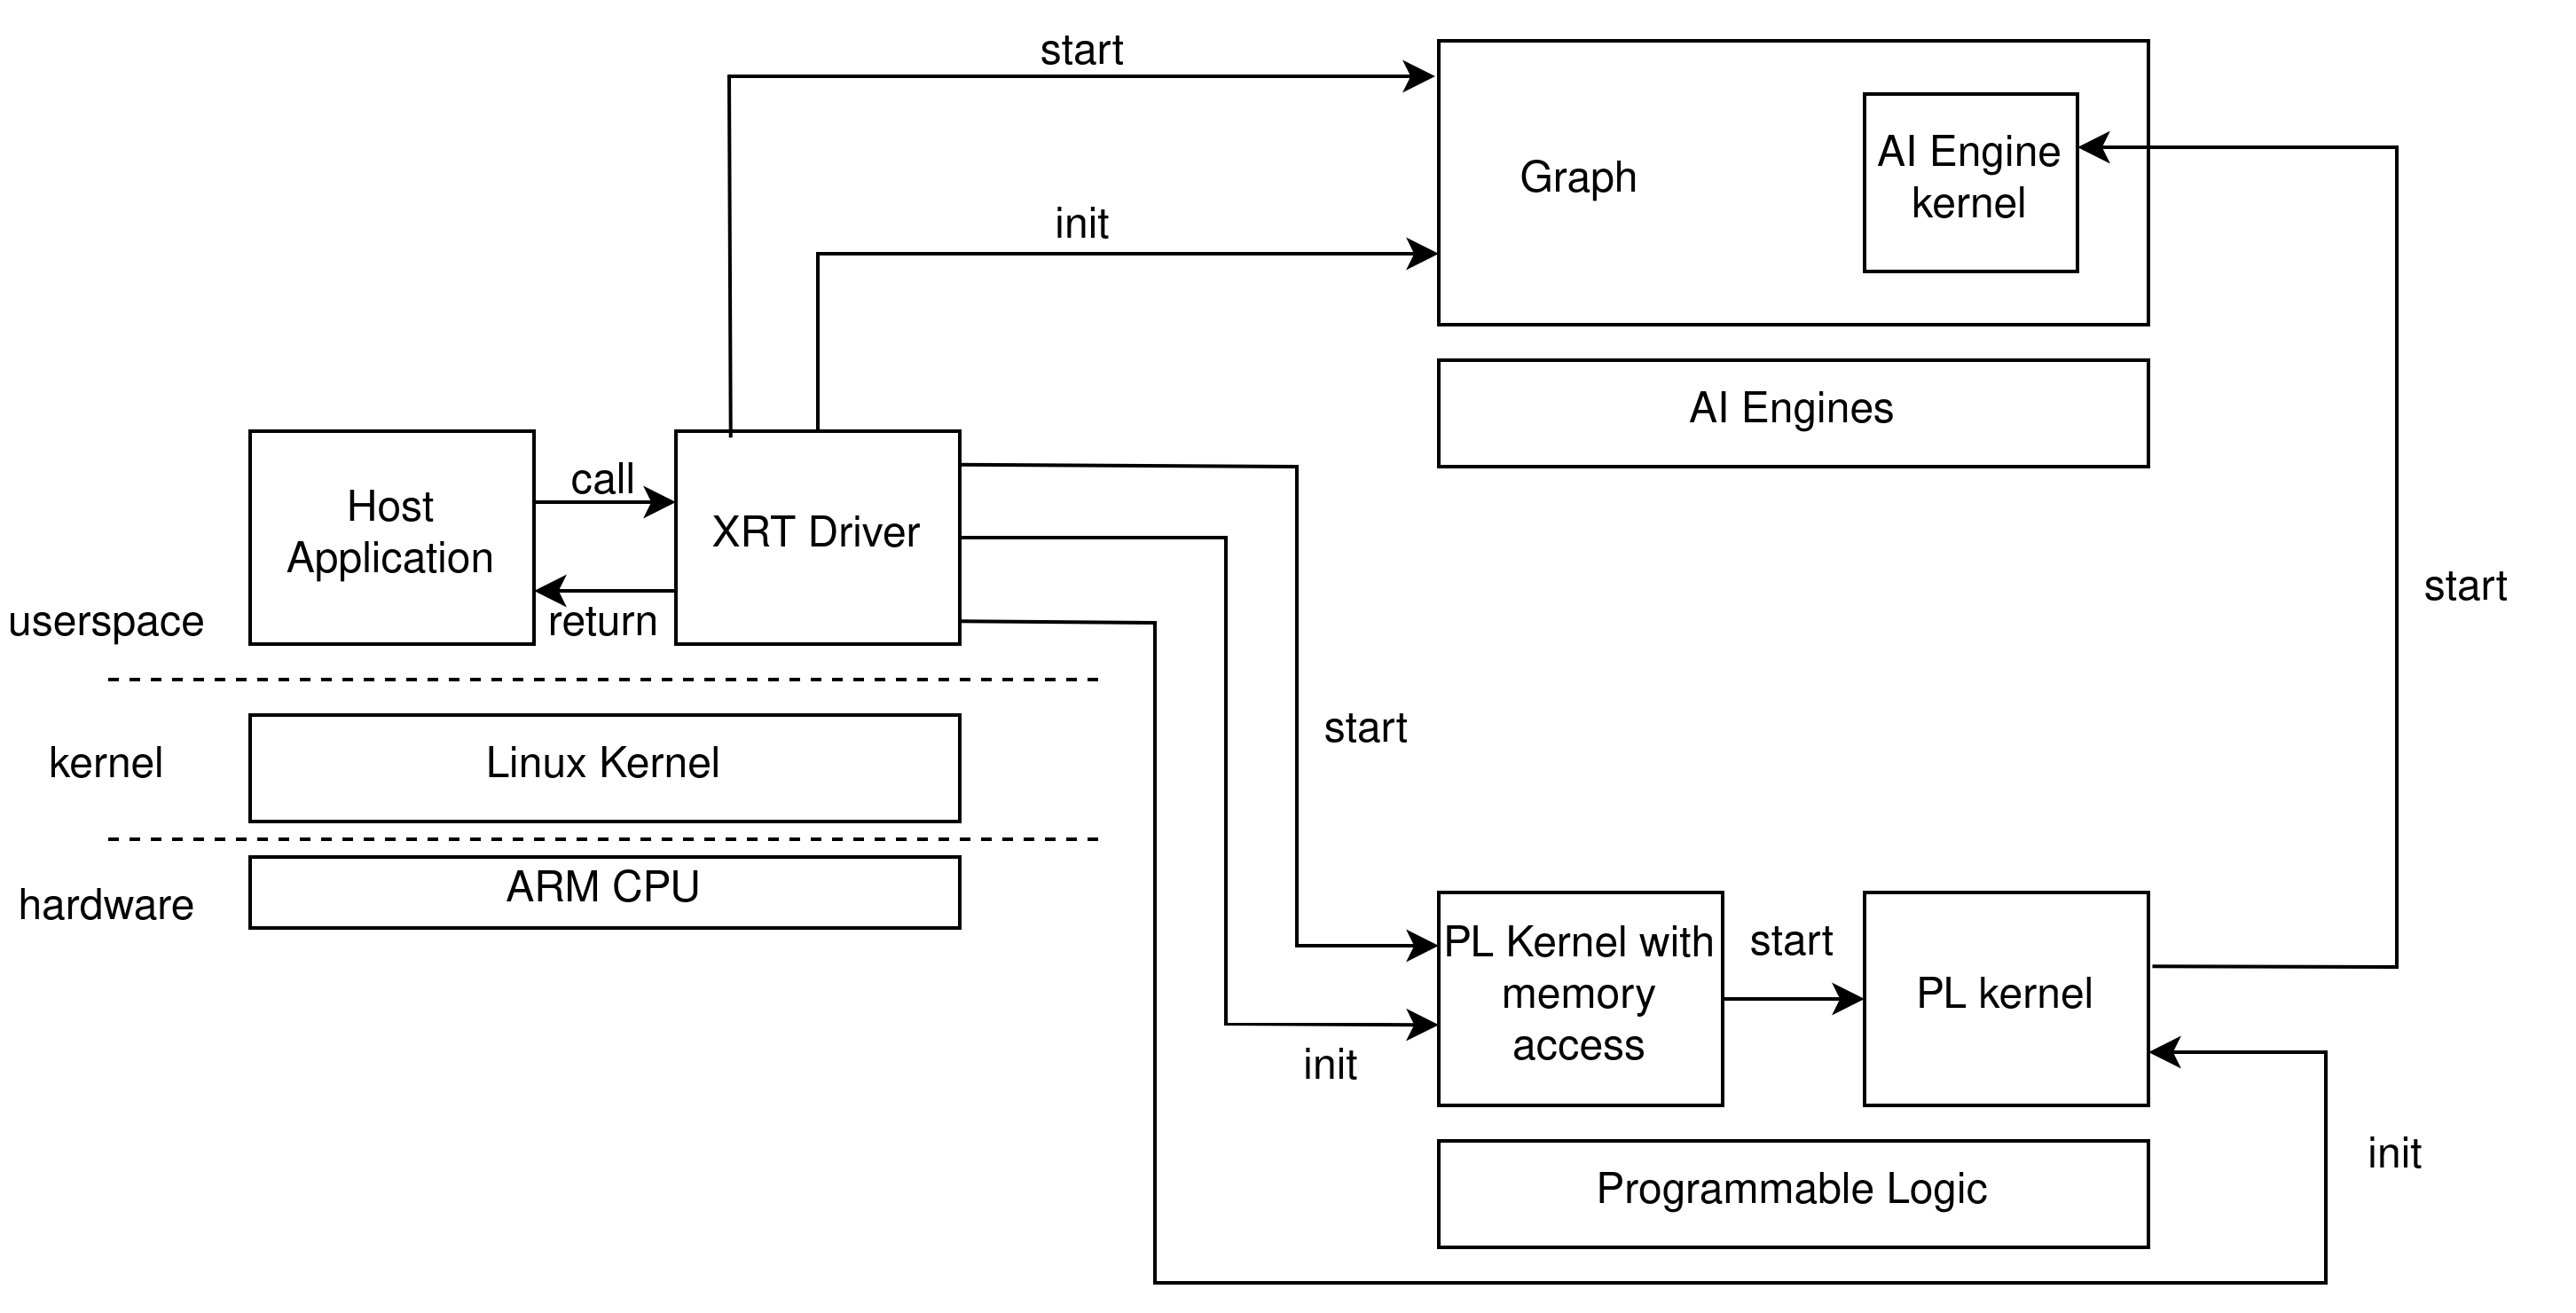
\includegraphics[width=1.0\textwidth]{images/host_interaction.png}
    \captionsetup{justification=centering}
    \caption{XRT Driver interaction scheme}
        This schematic shows the interaction of the host application with the XRT driver which enables the program flashed onto the PL and the AI Engines. Some specific functions are started from within the PL but are still initialised by the XRT driver.
    \label{fig:host_interact}
\end{figure}

%TODO add source for FFTW3, mersenne twister etc.
\section{Test data generation}
The generation of test data consists of two main parts: generating the real-valued input data and computing the expected results. For the input data generation, certain requirements must be met. The data should be randomly structured to avoid patterns that could favor a specific \ac{fft} algorithm. Although the data is random, it must also be reproducible to ensure comparability across tests. To achieve this, a random seed is generated using the \texttt{std::random\char`_device\char`_rd} function from the standard C++ library. This seed is stored to enable the generation of the same input data in future runs. The seed initializes the Mersenne Twister algorithm \texttt{std::mt19937}, an efficient pseudo-random number generator in C++ \cite{matsumoto_mersenne_1998}. This generator creates a consistent sequence of random numbers for a given seed. Each random number is transformed into a floating-point value between 0 and 100 using \texttt{std::uniform\char`_real\char`_distribution<float> dis(0, 100)}. These bounds are arbitrary and can be adjusted for different test cases. Each generated value is stored in a file, and a zero is added between each value to serve as the imaginary part, which is zero for a real-valued signal.\par
This file is then used to generate ground truth data by performing an \ac{fft} on it, which is done on an x86 \ac{cpu} using the FFTW3 library for C++. FFTW3 is a highly optimized library for fast \ac{fft} implementations across multiple platforms \cite{frigo_design_2005}, making it an ideal choice for generating this test case.\par
All generated data files are included in the package that is flashed onto the SD card, allowing them to be accessed directly on the Versal platform. 
